
%\documentclass{acm_proc_article-sp}
\documentclass[11pt,letterpaper]{article}

%==================================
% packages go here
%==================================

\usepackage{url}
\usepackage{graphicx}
\usepackage{cite} % sort citation numbers
\usepackage{color}
\usepackage{soul}
\usepackage{naaclhlt2012}
\usepackage{times}
\usepackage{latexsym}

%\usepackage{ntheorem}
%\usepackage{amsthm}
%\usepackage{multirow} % for complex tables
%\usepackage{times}
%\usepackage[pdftex]{hyperref}
%\hypersetup{colorlinks=false, pdfborder= 0 0 0}
%\usepackage[draft,inline,nomargin]{fixme}
%\newcommand{\hlfixme}[1]{\fixme{\hl{#1}}}
%\newcommand{\hlfxnote}[1]{\fxnote{\hl{#1}}}

%\newcommand{\name}{\emph{Watson Jr.}}
\newcommand{\name}{\emph{DeanQA~}}

\setlength\titlebox{6.5cm}    % Expanding the titlebox

%==================================

%\begin{document}

\title{\name: \\An Advanced Question Answering System}

\author{
	Yann Le Gall\\
    University of Pittsburgh\\	
	Department of Computer Science\\
	6503 Sennot Square\\
    {\tt ylegall@cs.pitt.edu}
\And
	Eric Heim\\
    University of Pittsburgh\\	
	5324 Sennot Square\\
    {\tt eth13@cs.pitt.edu}
	\\
\And
	Alex Conrad\\
    XYZ Company\\
    111 Anywhere Street\\
    Mytown, NY 10000, USA\\
    {\tt author1@xyz.org}
}

\date{12 December 2011}

\begin{document}

\maketitle

%==================================

%\begin{abstract}
%abstract goes here
%\end{abstract}

% A category with the (minimum) three required fields
%\category{I.2}{Artifical Intelligence}{Natural Language Processing}
%\terms{Algorithms, Experimentation}
%\keywords{Question Answering}

%==================================

\section{Introduction}
\label{sec:intro}

In this paper, we design, implement, and evaluate a question answering
(QA) system, \name. In our approach, we use several different strategies from
different domains to select potential answers. Then, we employ a
majority voting scheme to combine the results.

% TODO: should this description of the dataset go in another section?
To train and test our QA system, we used the ``CBC Reading
Comprehension Corpus''. This corpus is composed of 125 news stories,
each accompanied by a set of 6-10 factoid questions (e.g. questions
that begin with ``Who'', ``When'', ``Where'', etc.).
%The news stories were obtained from the ``CBC 4 Kids'' website,
%hosted by the Canadian Broadcast Corporation. The questions and an
%answer key were added by the MITRE Corporation, and are in the style
%of actual reading comprehension tests that are given to grade school
%children in the United States.

All stories in the dataset were been split into sentences (one
sentence per line) using the MXTERMINATOR sentence splitter developed
by Adwait Ratnaparkhi.  Paragraphs from the original story are
separated by an empty line. 

The rest of this paper is organized as follows: in
\S\ref{sec:implementation} we describe the design and implementation
of our QA system and each of its sub-components. Next, in
\S\ref{sec:evaluation} we evaluate our system on the test dataset and
present the performance results. Finally, we conclude in
\S\ref{sec:conclusion}.


\section{Implementation}
\label{sec:implementation}

In this section we discuss the design and implementation of \name
. First, we explain the general, overall structure. Then we give
a detailed description of the sub-components (\emph{AnswerFinders}) of
the system. Finally, we present our technique for combining the
potential answers from each sub-component.

\begin{figure*} 
	\centering
	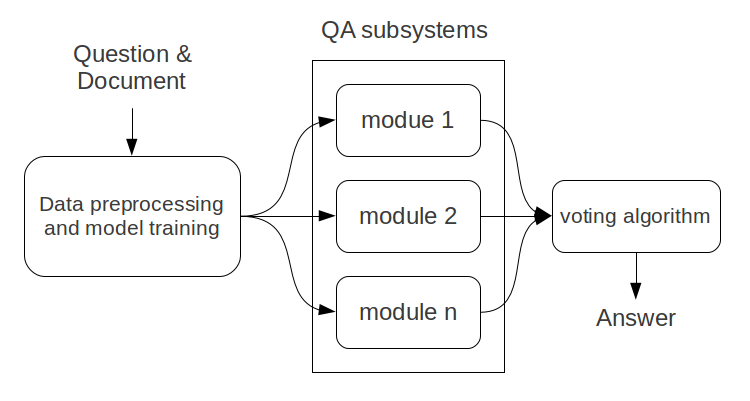
\includegraphics[width=0.7\textwidth]{model.png}
	\caption{The \name system model.}
	\label{fig:model}
\end{figure*}

Figure \ref{fig:model} shows the general design of \name.
The system takes processes a document and a set of questions as input.
At this point, several preprocessing steps might be performed,
including the removal of stop words, coreference resolution, etc.
Next, the processed document and the current question are passed to
each of the AnswerFinders. Each of these AnswerFinders implements a
different strategy for finding answers to the question, and they
each return a collection of \texttt{<answer,confidence>} pairs.
Finally, the potential answers are combineded in a voting algorithm
that gives different weights to the potential answers based on the
confidence and the question type.

In the next few subsections, we give more detailed descriptions of
the implementation of the different AnswerFinders and the
strategies that they use.

\subsection{Bag-of-Words}

The Bag-of-words (BOW) model is a simple model that provides
relatively good performance in our systeml. In our domain, BOW treats
each question as a set of words. Then, for each sentence in the
document, we count the number of matching words. The probability that
a sentence is the correct answer is estimated as the ratio of the
number of matching words to the total possible number of matches.

\subsection{Linguistic Rule-based Strategies}

We also implemented a rule-based AnswerFinder based on the previous
work of \cite{riloff2000}. This system applies different rules based
on the question type. A preliminary score is calculated for each line
based on the BOW model. Then, different amounts of points are awarded
for each satisfied rule.

\subsection{NLP Components}

% TODO: Alex writes this

\subsection{SVM Classification}
\paragraph{}
The last component of the \name system takes a Machine Learning approach that barrows heavily 
from the work done by \cite{Ng00amachine}.  In their paper, the authors extracted features from a training
set of news documents and corresponding questions about the documents.  Then, they trained a C5 
decision tree classifier, which is a more recent version of the C4.5  \cite{Quinlan:1993:CPM:152181} classifier, 
in order to predict which sentence answers a question.  Each data point represents a sentence-question pair with a 
label being positive (1) for sentences that answer the paired question or negative (-1) 
for sentences that do not.

Each feature represents some characteristic of the sentence, the question, or both.  
For example, the Diff-from-Max-Word-Match (DMWM) gives a score based on how many lemmatized 
words are in both the sentence and question.  This is very similar to the bag of words component. 
 Other features take advantage of named entity recognition, whether the sentence is the title or dateline, 
or keywords that were learned to be commonly present in sentences that answer specific question types. 
 All of the features from \cite{Ng00amachine} were used except for the ``keywords in questions'' features,
 as well as the coreference information to boost the named entity features.  For a more detailed explanation 
 of these features, see their work.  We used the Stanford CoreNLP library for part of speech tagging 
 \cite{Toutanova00enrichingthe} and named entity recognition \cite{Finkel05incorporatingnon-local} in the feature extraction
 process.  In addition to the features mentioned previously, we added binary features 
 to describe the question type.  More specifically, six binary features were added indicating whether the question 
 for the data point was a ``Who'', ``What'', ``Where'', ``When'', ``Why'', or ``How'' question.  If none of 
 the features were ``true'' then the question type could be interpreted as ``Other''.   In total, 24 features 
 were extracted.

 The main difference this component has from \cite{Ng00amachine} is that instead of using the C5 classifier, 
 we trained a Support Vector Machine (SVM).  We used the WEKA 3.6 \cite{Hall_theweka} Java wrapper 
 class for the LibSVM 3.11 \cite{Chang01libsvm:a} SVM library to implement this SVM.  The 
 radial basis kernel was used with a cost parameter of 4.5 and a gamma parameter of 1/24 (1 over the number 
 of features) after cross validation.   This model was trained on the ``input'' dataset, which had 37 documents 
 and 324 questions.  On the ``input-test1'' set (36 documents, 310 questions) we found that using the WEKA 
 implementation of the C4.5 classifier (called J48, parameters M = 7, N = 17) resulted in having a lower 
 prediction accuracy (131 out of 310) than the SVM model (148 out of 310).

% TODO: Eric writes this part

\subsection{Combining Answers with Majority Voting}
Previous work by Rotaru and Litman demonstrates that combining
the outputs of multiple QA systems can achieve better results than the
individual systems alone \cite{rotaru2005}. We incorporate this idea
into the design of our QA system by combining the outputs from each of
the subsystems described above.

% TODO: describe how we combine the different results

\section{Evaluation}
\label{sec:evaluation}

%******************************************************************
%Accuracy: 181 correct out of 310 questions - 58.39%.
%******************************************************************
%NORMALIZED ACCURACY : 60.89%

\begin{table}
\centering

	\begin{tabular}{|r|c|c|}
	\hline
	Type   & \# Correct & Percentage \\
	\hline
	\hline
	WHEN   &  25 out of  34 &  73.53\% \\
	\hline
	WHERE  &  23 out of  36 &  63.89\% \\
	\hline
	WHAT   &  42 out of  80 &  52.50\% \\
	\hline
	WHY    &  26 out of  44 &  59.09\% \\
	\hline
	WHO    &  26 out of  41 &  63.41\% \\
	\hline
	HOW    &  36 out of  68 &  52.94\% \\
	\hline
	OTHER  &   3 out of   7 &  42.86\% \\
	\hline
	\hline
	TOTAL  & 181 out of 310 &  58.39\% \\
	\tiny{NORMALIZED}  &  &  60.89\% \\
	\hline
	\end{tabular}

\caption{Statistics by question type.}
\label{table:question-types}
\end{table}

%
%WHEN   :   25 out of   34 -  73.53\%
%WHERE  :   23 out of   36 -  63.89\%
%WHAT   :   42 out of   80 -  52.50\%
%WHY    :   26 out of   44 -  59.09\%
%WHO    :   26 out of   41 -  63.41\%
%HOW    :   36 out of   68 -  52.94\%
%OTHER  :    3 out of    7 -  42.86\%
%TOTAL  :  181 out of  310 -  58.39\%
%TOTAL  & 181 out of 310 &  58.39\% \\
%




\section{Conclusions}
\label{sec:conclusion}

Question-answering is complex task and a cutting-edge research area
in natural language processing. 


%ACKNOWLEDGMENTS are optional
%\section{Acknowledgments}

%\bibliographystyle{abbrv}
%\bibliographystyle{plain}
\bibliographystyle{naaclhlt2012}
%\bibliographystyle{acl}
\bibliography{references} 

%
%\appendix
%%Appendix A
%\section{Headings in Appendices}
%\balancecolumns


\end{document}

